\documentclass[lang=cn]{elegantpaper}
\usepackage{listings}
\usepackage{hyperref}
\usepackage{graphicx}
\title{编译原理 -- 实验 1 - 词法分析}
\author{61519322 杨哲睿}
\date{\today}

\begin{document}

\maketitle

\tableofcontents


% 提交清单:
% - Mini语言的词法规则描述(正规式或正规文法)
% - 正规式或正规文法->NFA->DFA->minimized DFA的手工过程(拍照整理为word或pdf文档)
% - 词法分析程序
% - 测试用例文件和测试结果文件
% - 实验报告

% 选择语言:pascal
% 源语言: rust-lang

\section{引言}

\subsection{实验要求}

\begin{quote}
    选择一个你熟悉的程序设计语言,找到它的规范(referrence or standard)。在规范中找到其词法的BNF或正规式描述。
\end{quote}

\begin{remark}
    选择的程序设计语言为:\lstinline|pascal|(源语言),具体规范参考为 \hyperref{https://github.com/bonzini/flex/blob/master/examples/manual/pascal.lex}{}{}{Github-pascal词法的lex描述}。
\end{remark}

\begin{quotation}
    选择该语言的一个子集(能够构成一个mini的语言,该语言至少能够进行函数调用、控制流语句(分支或循环)、简单的运算和赋值操作。)给出该mini语言的词法的正规文法或正规式。
    
\end{quotation}

在这里,选择的mini语言关键字为:

\begin{lstlisting}[language=pascal]
and
begin
div
do
else
end
for
function
if
in
nil
not
of
procedure
program
repeat
set
then
to
until
var
while
\end{lstlisting}
与标识符一同识别。

relop 如下:

\begin{lstlisting}[language=pascal]
<= >= < > <> =
:=
..
+ - * /
\end{lstlisting}

界符 sep 如下:
\begin{lstlisting}[language=pascal]
[ ] ( )
, ; .
\end{lstlisting}

其他需要的基本词法单元如下:
\begin{enumerate}
    \item 数
    \item 字符串
\end{enumerate}

下面给出具体的词法规则描述。

\section{词法规则描述、Minimized-DFA 简化过程}

如图所示:
% TODO:  required
\begin{figure}
	\centering
	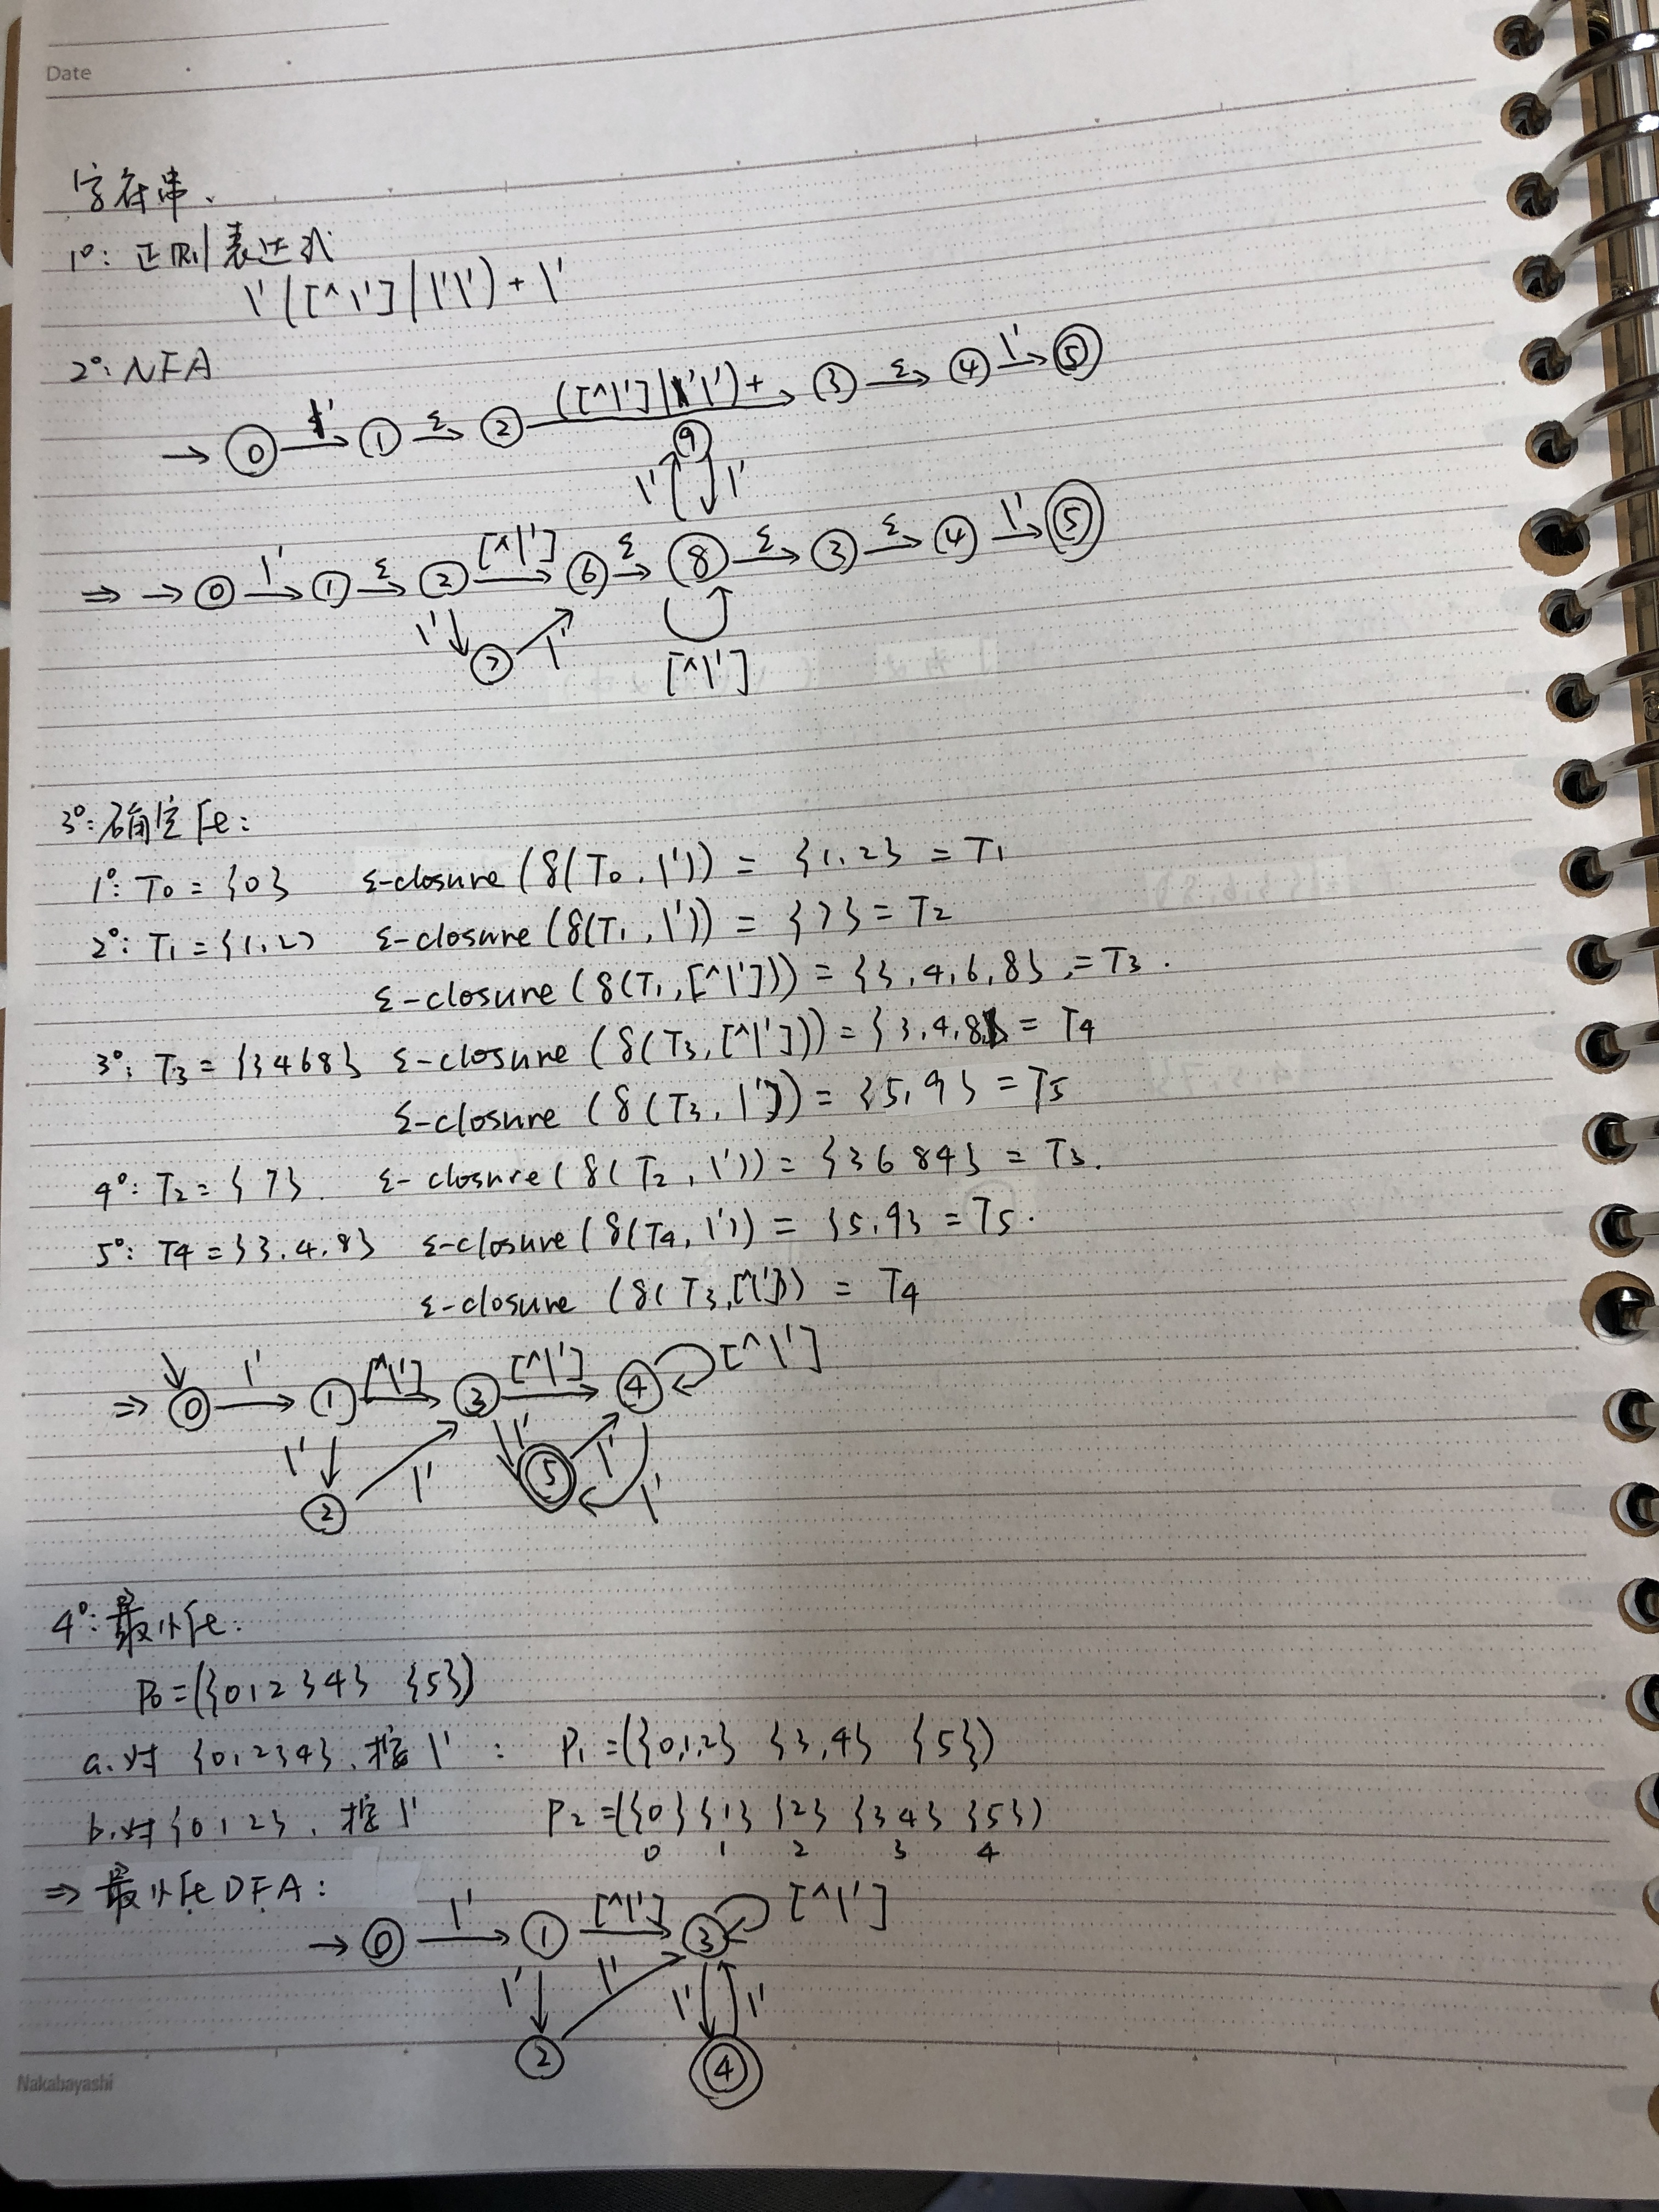
\includegraphics[width=0.7\linewidth]{img/IMG_3153}
	\caption{字符串}
	\label{fig:img3153}
\end{figure}
\begin{figure}
	\centering
	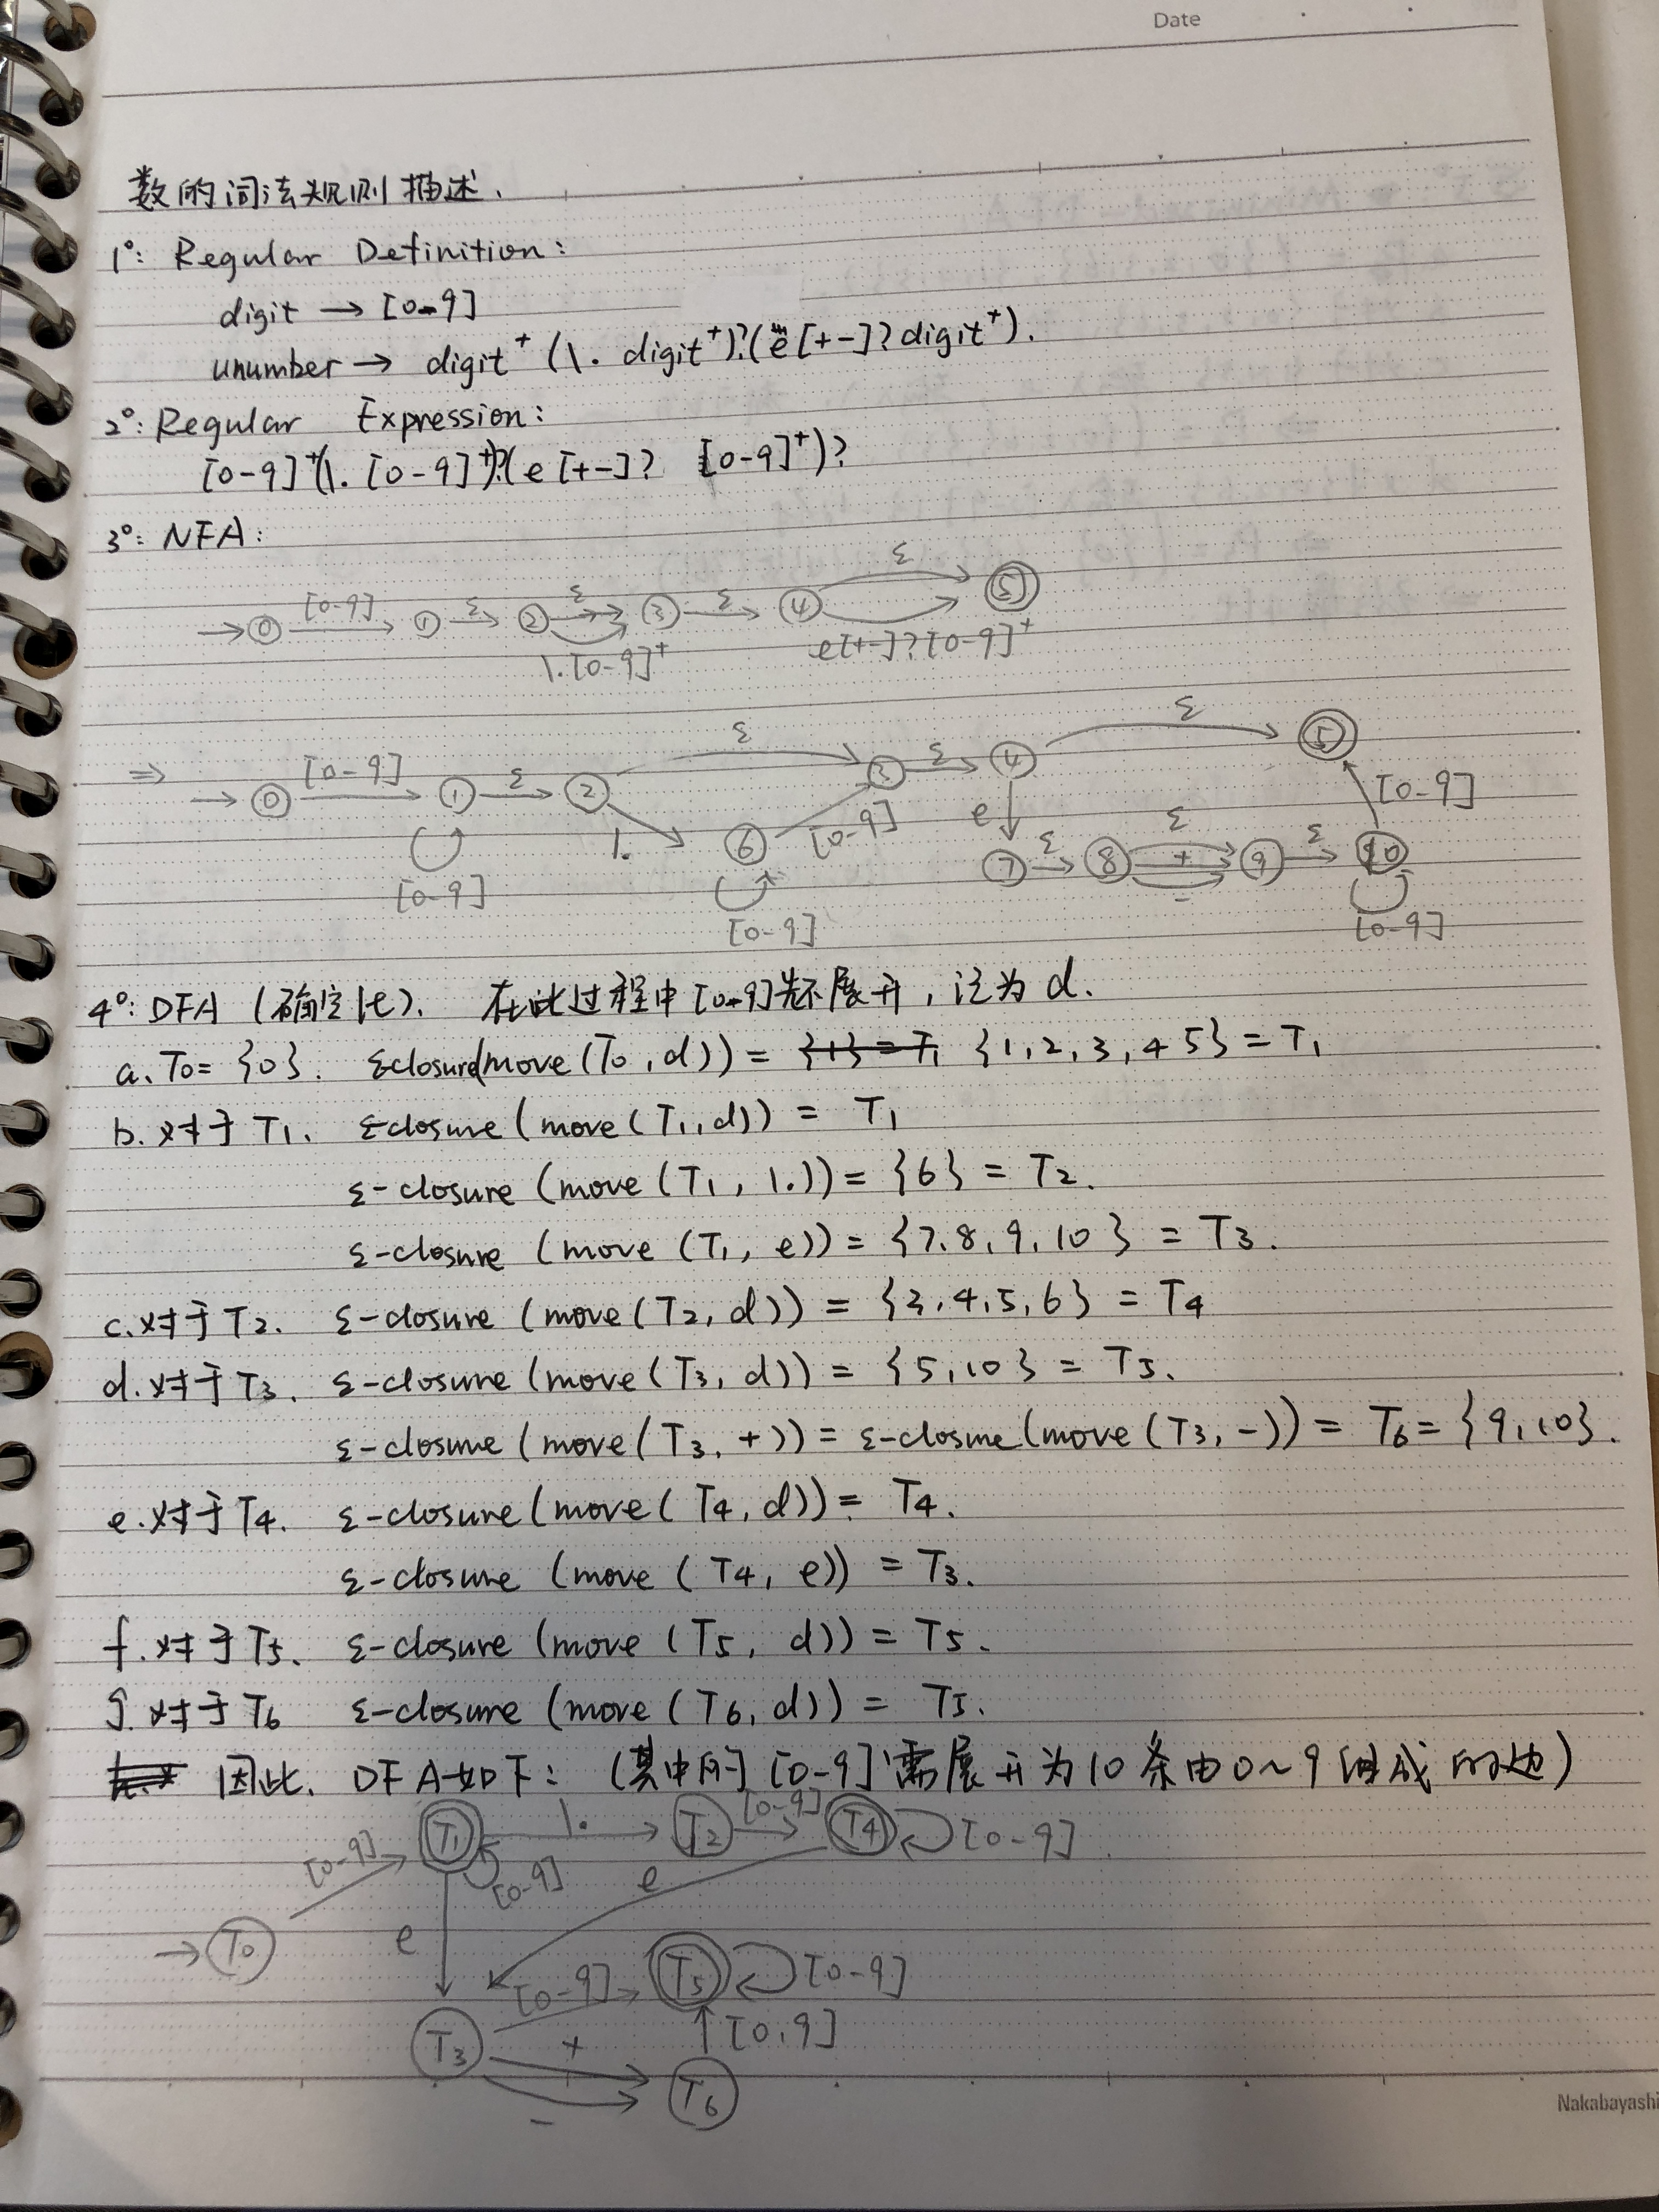
\includegraphics[width=0.7\linewidth]{img/IMG_3154}
	\caption{数字识别1}
	\label{fig:img3154}
\end{figure}

\begin{figure}
	\centering
	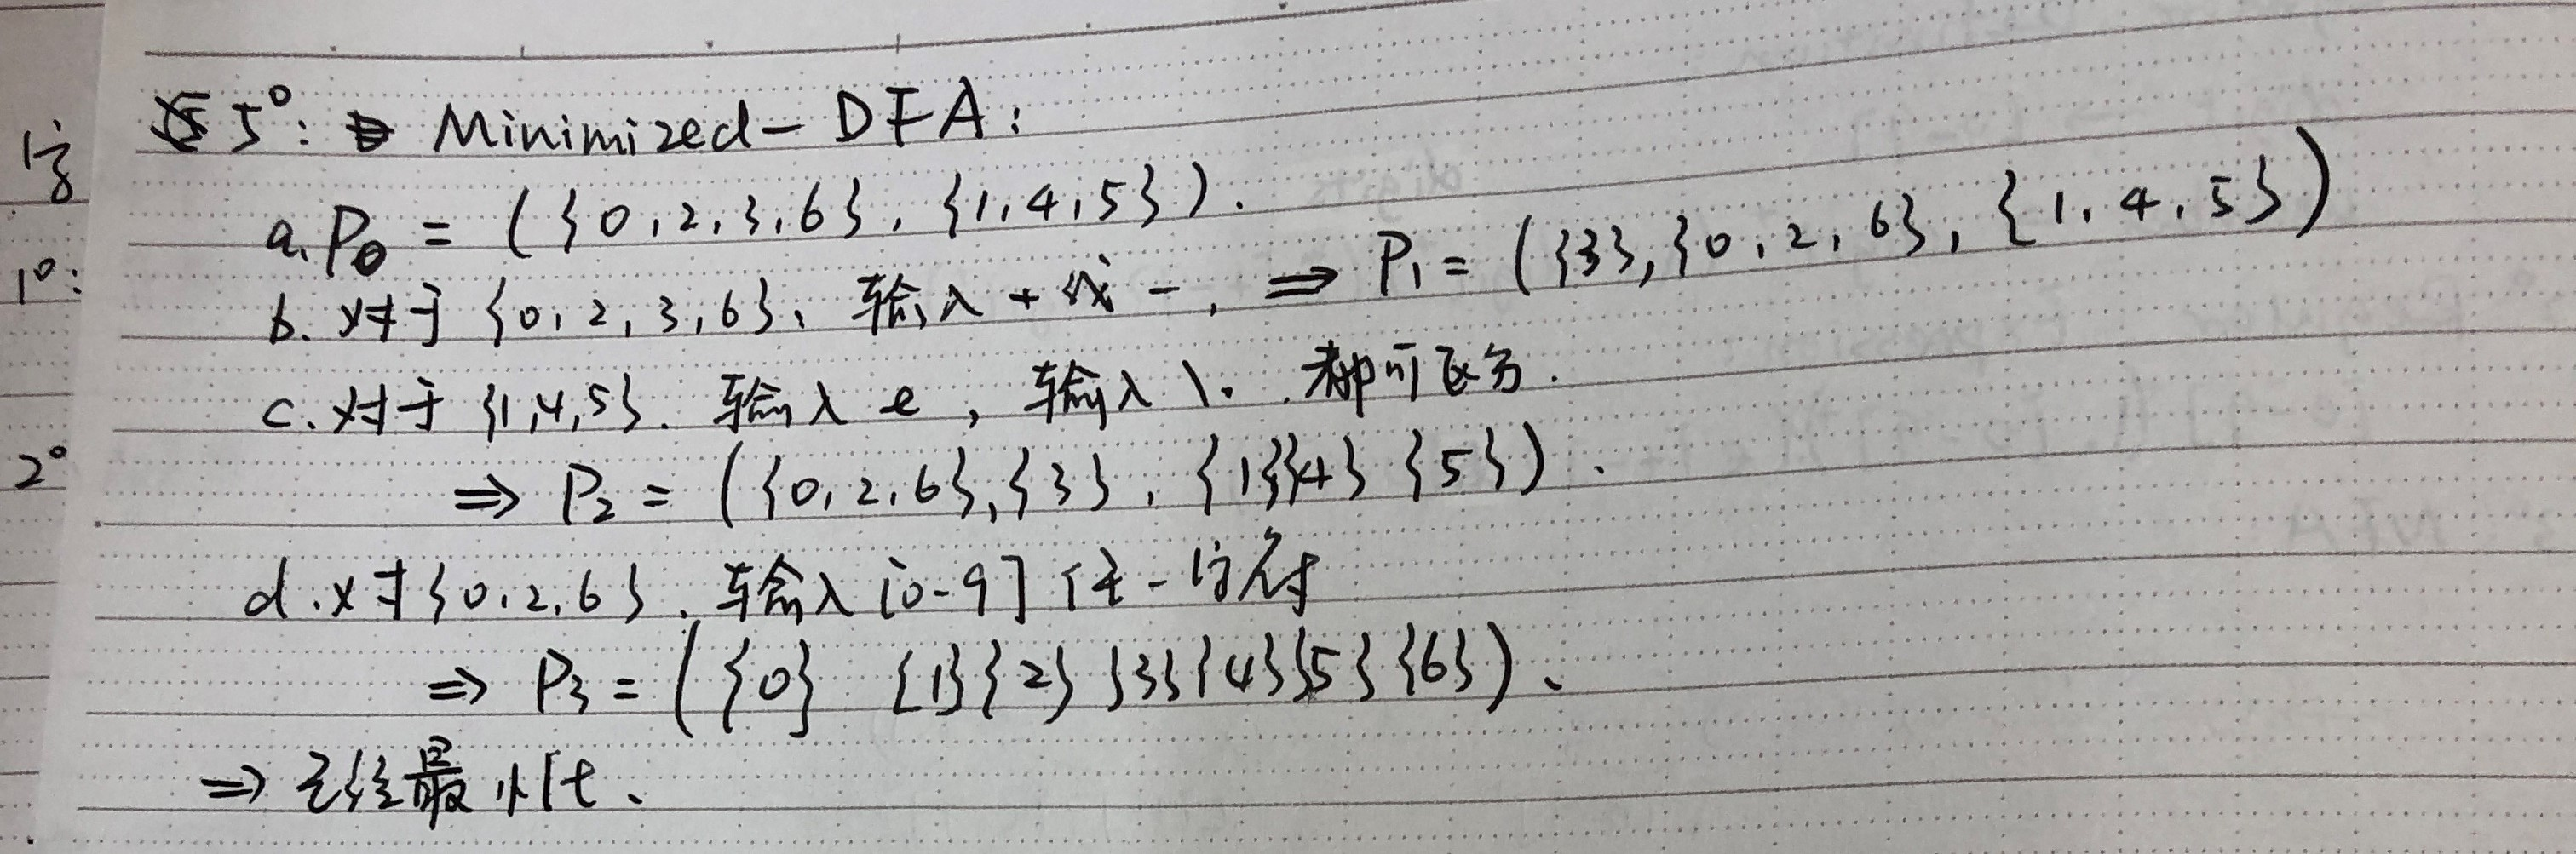
\includegraphics[width=0.7\linewidth]{img/IMG_3155}
	\caption{数字识别2}
	\label{fig:img3155}
\end{figure}

\begin{figure}
	\centering
	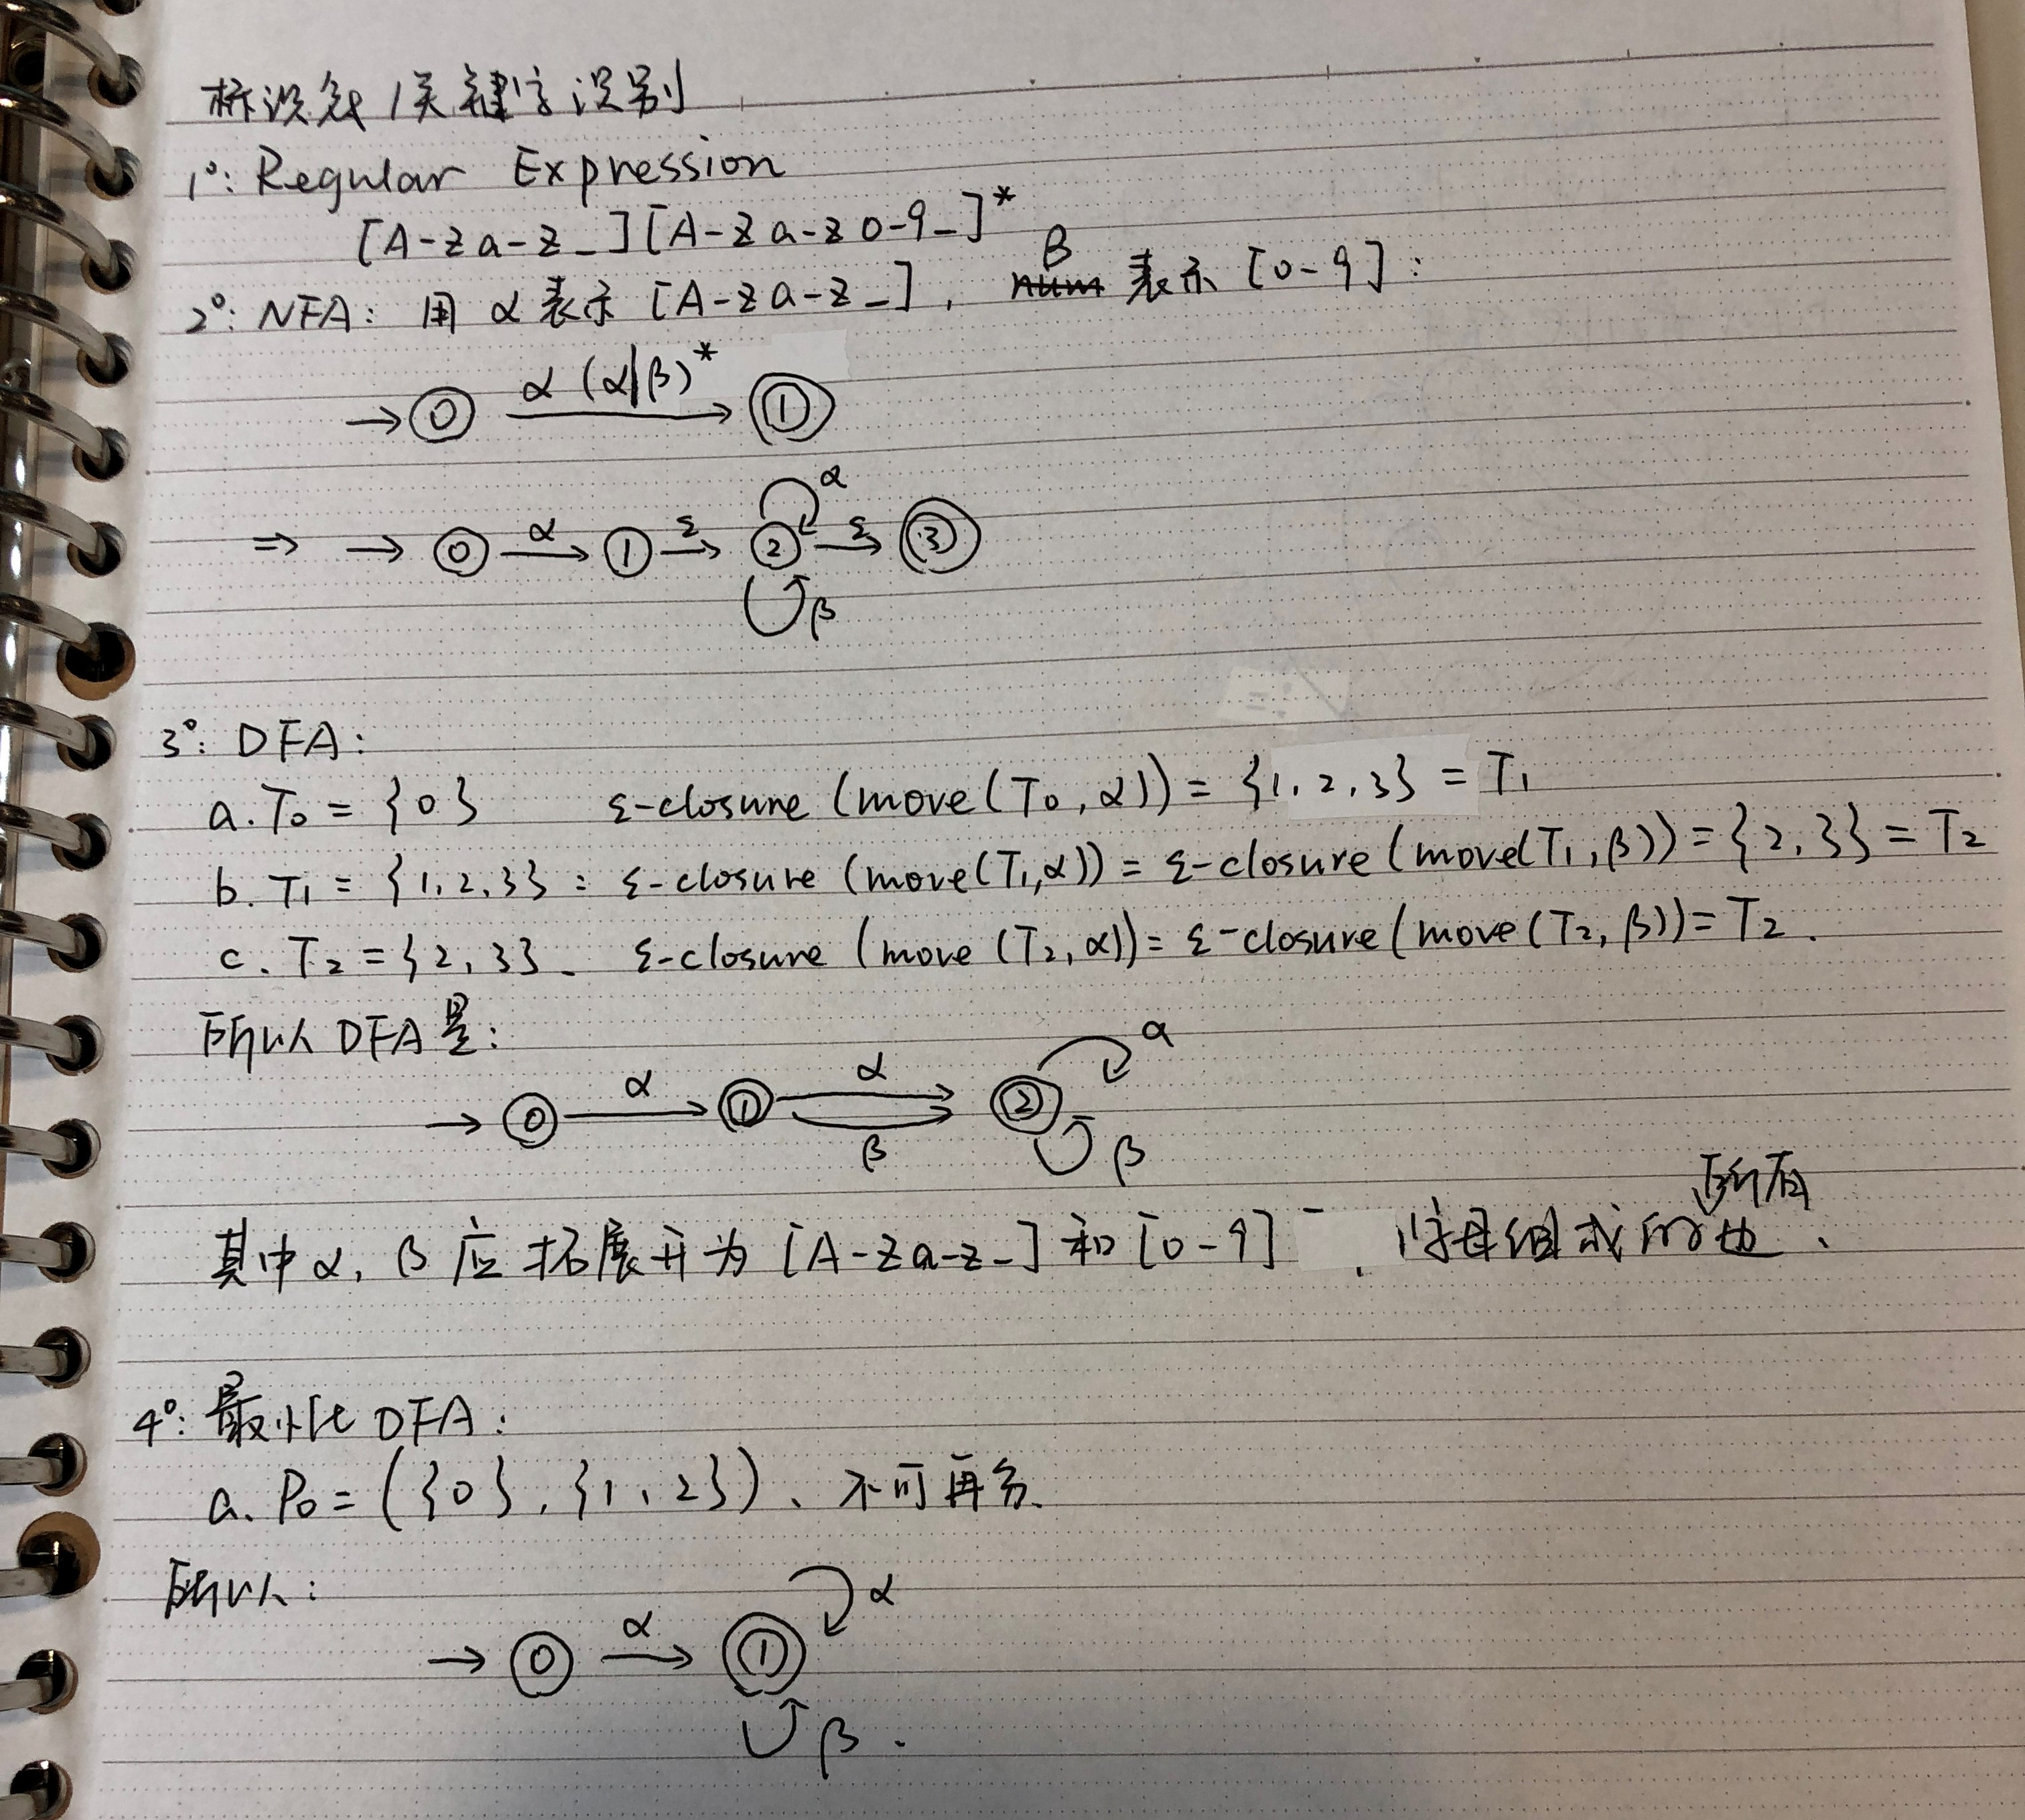
\includegraphics[width=0.7\linewidth]{img/IMG_3156}
	\caption{标识符/关键字识别}
	\label{fig:img3156}
\end{figure}

\begin{figure}
	\centering
	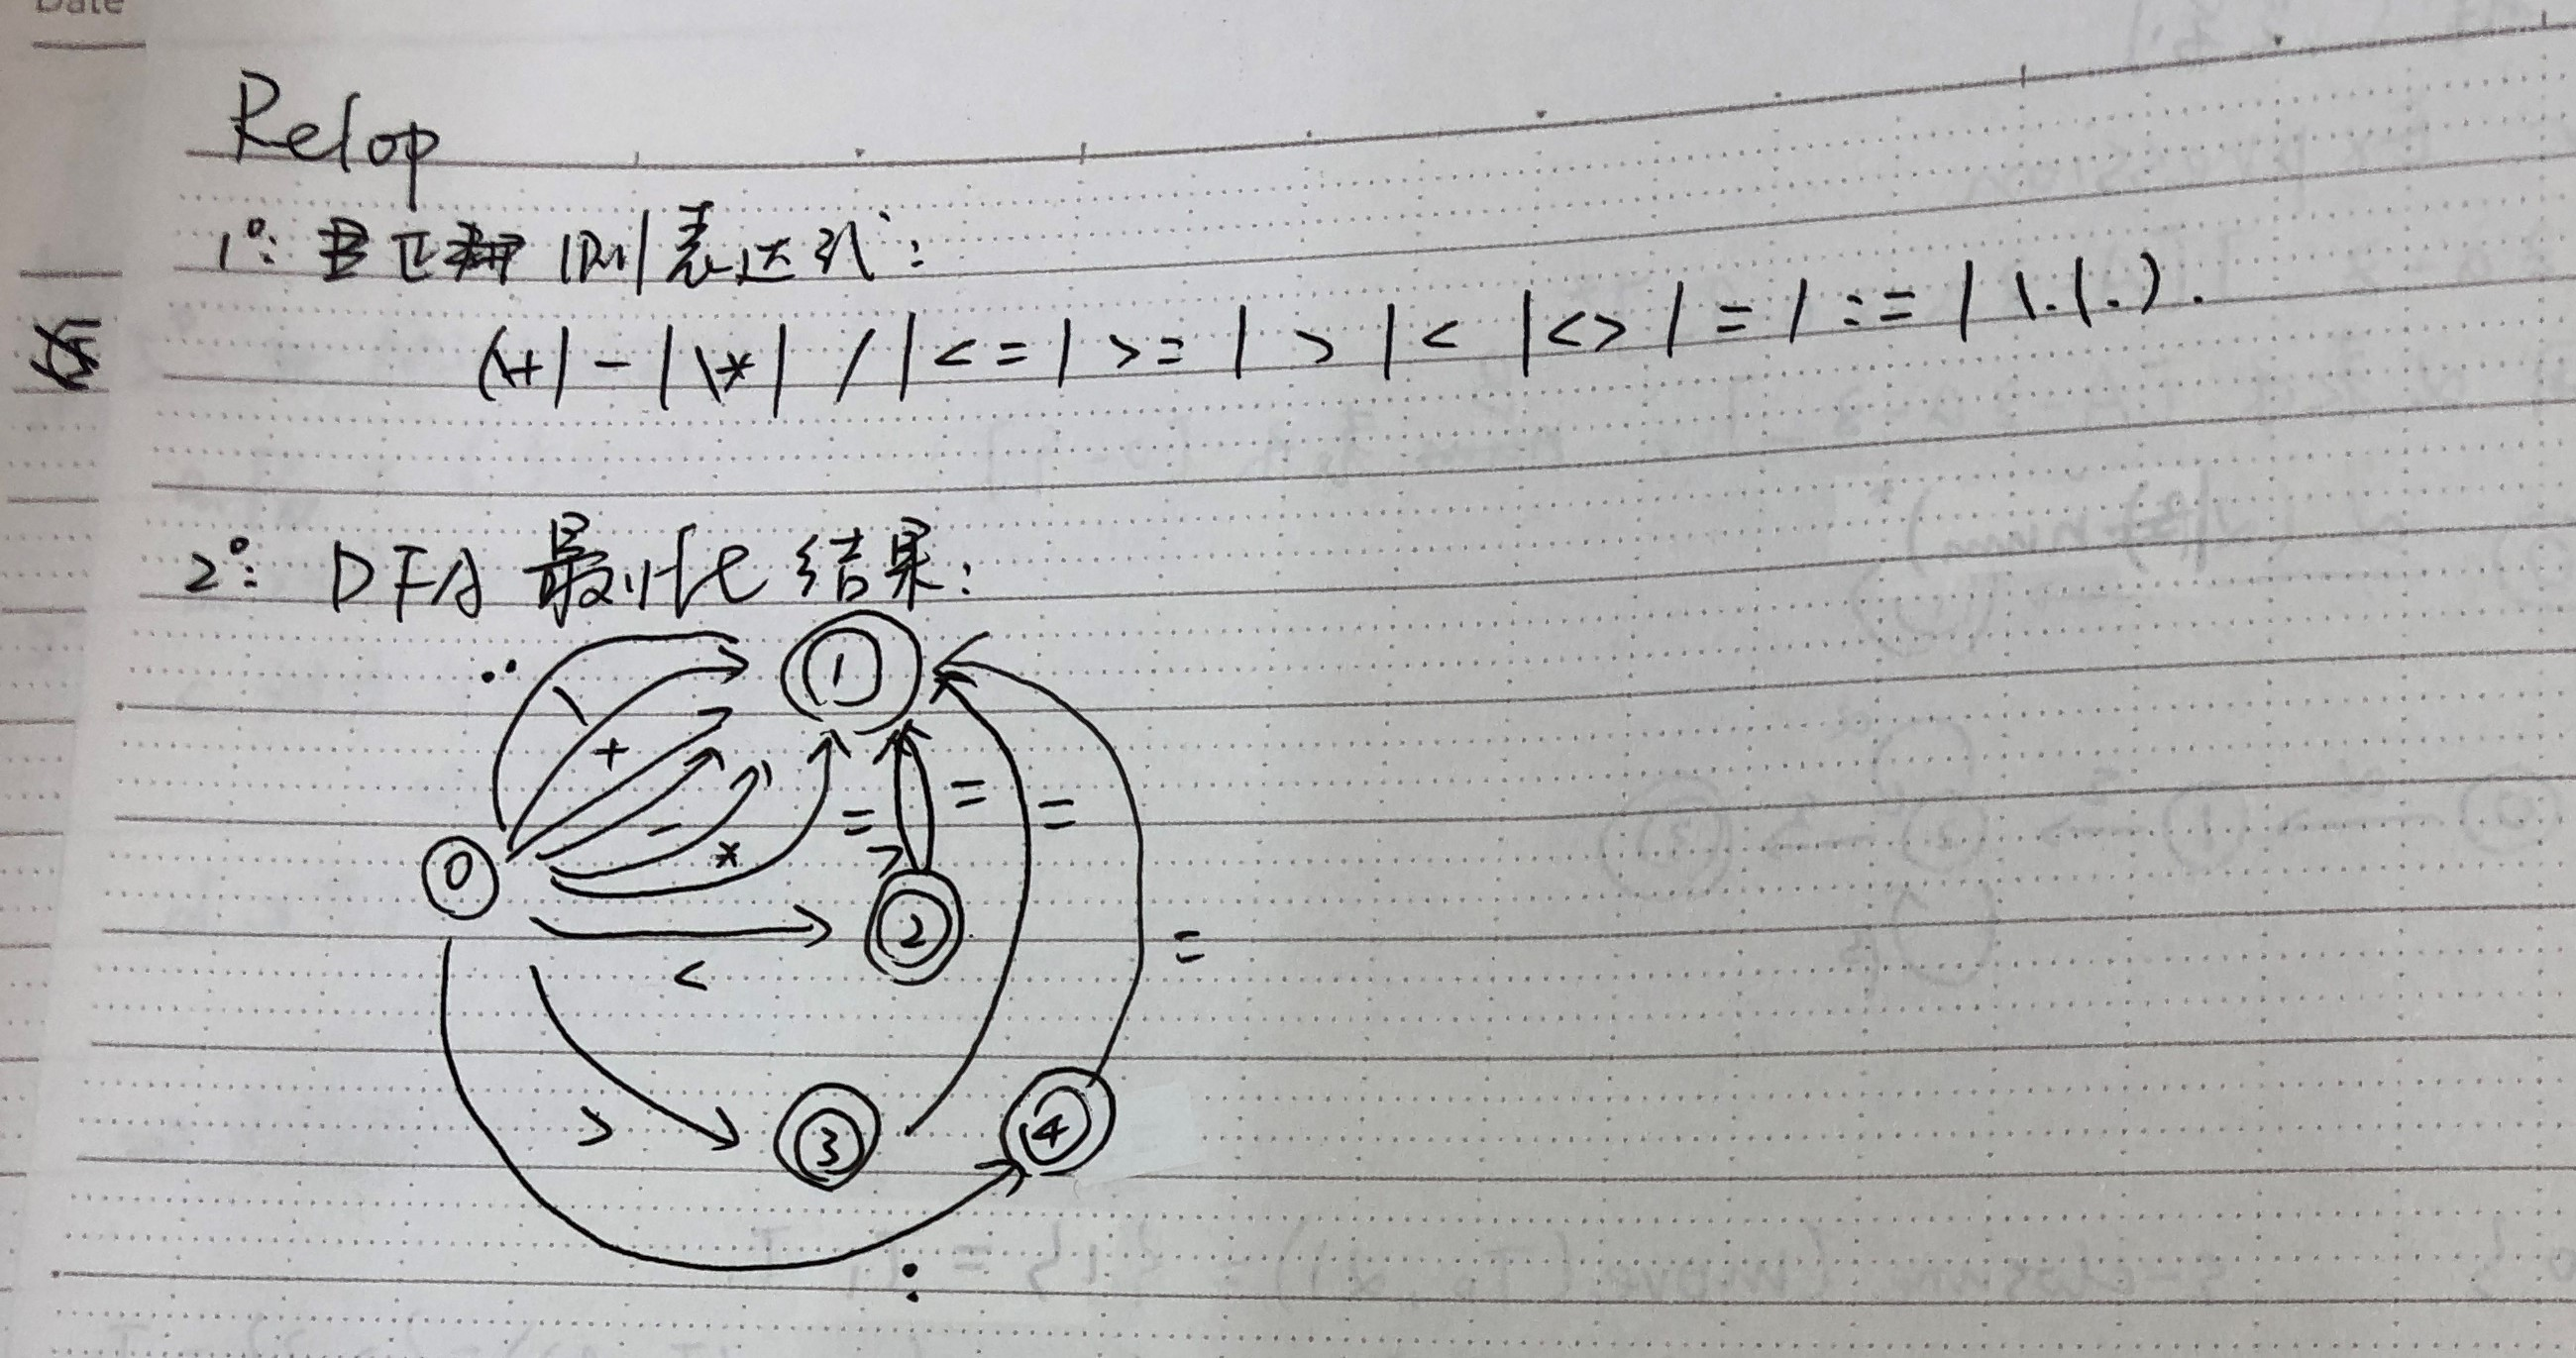
\includegraphics[width=0.7\linewidth]{img/IMG_3157}
	\caption{Relop识别}
	\label{fig:img3157}
\end{figure}


\section{词法分析程序}


\subsection{简述}

正如DFA的定义:描述DFA只需要五元组 $S = (K, \Sigma, f, S, Z)$。那么描述DFA中的状态
只需要状态转换函数:
$$
change_{S}(\mathrm{ch}) = f( S, \mathrm{ch})
$$
这适合于将函数作为第一公民的{\textbf{函数式编程}}来实现。同时,对于$change_S(\mathrm{ch})$
做出如下的约定:

\noindent $change_{S} (\mathrm {ch}) = $
\begin{enumerate}
    \item 若DFA中存在 $S' = f (S, \mathrm{ch})$ 那么输出为对应状态(的状态转换函数)
          即输出为$change{S'}$
    \item 若DFA中不存在这样的转换,那么若
        \subitem $S \in Z$ 输出 \lstinline|true|;
        \subitem $S \notin Z$ 输出 \lstinline|false|。
\end{enumerate}

例如:

\begin{example} 字符串的识别:

    正如上文所提到的,将手工简化好的DFA转换为代码,即为:

\begin{lstlisting}[language=lisp,caption=Racket-lang 实现-用于匹配字符串的DFA定义]
; DFA -- string
(define StringSM
(let ([q? (lambda (ch) (char=? ch #\'))])
    (letrec ([s0 (lambda (ch) (cond
                                [(q? ch) s1]
                                [else #f]))]
             [s1 (lambda (ch) (cond
                                [(q? ch) s1]
                                [(char=? #\nul ch) #f]
                                [else s3]))]
             [s2 (lambda (ch) (cond
                                [(q? ch) s3]
                                [else #f]))]
             [s3 (lambda (ch) (cond
                                [(q? ch) s4]
                                [(char=? #\nul ch) #f]
                                [else s3]))]
             [s4 (lambda (ch) (cond
                                [(q? ch)s3]
                                [else #t]))])
    s0)))
\end{lstlisting}

    与此同时,为了运行该自动机,完成了\lstinline|iter-until-fail|函数,该函数的作用是
    在给定的符号列上运行DFA,直到DFA无法识别当前符号时停止。

\begin{lstlisting}[language=lisp, caption=在给定的符号列上,运行该状态机]
(define (iter-until-fail s l)
  (let* ([ch (if (empty? l)
                 #\null
                 (first l))] ; getch --> ch
         [t (s ch)])         ; transition {s --[ch]-> t}
    (if (boolean? t)         ; stop?
        (if t
            (list)           ; '()  -> accept
            (void))          ; void -> fail
        (let ([result (iter-until-fail t (rest l))])
          (if (void? result)
              (void)         ; -> fail matching
              (cons ch result))
          ))))
    \end{lstlisting}
\end{example}

\subsection{实现细节}

\subsubsection{标识符-关键字的特殊处理}

正如龙书中所说的,一般而言,关键字的识别可以通过在识别出一个标识符之后进行后处理,判断各个
标识符是否是关键字,如果是关键字那么就返回关键字,反之判定为标识符。

\subsubsection{数组大小约定的数字识别 -- 向前看}

一个特情况是这样的:

\begin{lstlisting}[language=pascal]
var a: array [1..4] of int;
\end{lstlisting}

考虑 \lstinline|1..4| 的判断,首先看\lstinline|1|,得到的是需要做数字的匹配。在第二个 \lstinline|.| 
处无法进行识别。且第一个识别出的\lstinline|1.|实际语义是错误的。因此需要另外识别,即如果判断到数字、以 
\lstinline|.| 结尾,且下一个紧接的是 \lstinline|.|,那么识别为数组大小约定的 \lstinline|..|。

\subsection{词法分析函数 \lstinline|get-token|}

\begin{lstlisting}[language=lisp]
(define (get-token str)
  (let* ([buffer (string->list str)]
         [s (first buffer)]) ; s: the first char in buffer
    (cond
      ; Matching whitespace
      [(ws? s)
       (let ([matched (Whitespace! buffer)])
         (token (list->string matched) token-whitespace (void)))]
      ; Matching seperator
      [(try-sep s)
       (token (list->string (list s)) token-sep (try-sep s))]
      ; Matching numbers
      [(digit? s)
       (let ([matched (Number! buffer)])
         (if (void? matched)
             ; Look Forward.
             (let ([matched (ArrayIndex! buffer)])
               (if (void? matched)
                   (void)
                   (if (and
                        (>= (string-length str) (+ 2 (length matched)))
                        (string=? ".." (substring str (length matched) (+ 2 (length matched)))))
                       (token (list->string matched) token-number (void))
                       (void))))
             (token (list->string matched) token-number (void))
             ))]
      [(relop-letter? s)
       (let ([matched (Relop! buffer)])
         (if (void? matched)
             (void)
             (let ([content (list->string matched)])
               (token content token-relop (try-relop content)))))]
      ; Matching identifier/keyword
      [(letter_? s)
       (let ([matched (Identifier! buffer)])
         (if (void? matched)
             (void)
             (let* ([content (list->string matched)]
                    [kw (try-keyword content)])
               (if kw
                   (token content token-keyword kw)
                   (token content token-identifier content))
               )))]
      [(char=? #\' s)
       (let ([matched (String! buffer)])
         (if (void? matched)
             (void)
             (let ([content (list->string matched)])
               (token content token-string content))))]
      [else (println "Error.")])))
\end{lstlisting}

\subsection{测试用例和测试结果}

\subsubsection{测试1 -- 数字、字符串、标识符}

测试用例如下:

\lstinputlisting[language=pascal, caption={test1.pas}]{../lex/test1.pas}

测试结果如下:

\begin{lstlisting}
Content of test1.pas is:
a := b + 1;
c = '123';
i0123_abc
'3124''123'
1.3245
1e3
1e-3
1.0e3
13
-13

################## RESULT OF LEXER ##################

#(struct:token a #<token-kind:token-identifier> a)
#(struct:token <whitespace> #<token-kind:token-whitespace> #<void>)
#(struct:token := #<token-kind:token-relop> assign)
#(struct:token <whitespace> #<token-kind:token-whitespace> #<void>)
#(struct:token b #<token-kind:token-identifier> b)
#(struct:token <whitespace> #<token-kind:token-whitespace> #<void>)
#(struct:token + #<token-kind:token-relop> plus)
#(struct:token <whitespace> #<token-kind:token-whitespace> #<void>)
#(struct:token 1 #<token-kind:token-number> #<void>)
#(struct:token ; #<token-kind:token-sep> semicolon)
#(struct:token <whitespace> #<token-kind:token-whitespace> #<void>)
#(struct:token c #<token-kind:token-identifier> c)
#(struct:token <whitespace> #<token-kind:token-whitespace> #<void>)
#(struct:token = #<token-kind:token-relop> eq)
#(struct:token <whitespace> #<token-kind:token-whitespace> #<void>)
#(struct:token '123' #<token-kind:token-string> '123')
#(struct:token ; #<token-kind:token-sep> semicolon)
#(struct:token <whitespace> #<token-kind:token-whitespace> #<void>)
#(struct:token i0123_abc #<token-kind:token-identifier> i0123_abc)
#(struct:token <whitespace> #<token-kind:token-whitespace> #<void>)
#(struct:token '3124''123' #<token-kind:token-string> '3124''123')
#(struct:token <whitespace> #<token-kind:token-whitespace> #<void>)
#(struct:token 1.3245 #<token-kind:token-number> #<void>)
#(struct:token <whitespace> #<token-kind:token-whitespace> #<void>)
#(struct:token 1e3 #<token-kind:token-number> #<void>)
#(struct:token <whitespace> #<token-kind:token-whitespace> #<void>)
#(struct:token 1e-3 #<token-kind:token-number> #<void>)
#(struct:token <whitespace> #<token-kind:token-whitespace> #<void>)
#(struct:token 1.0e3 #<token-kind:token-number> #<void>)
#(struct:token <whitespace> #<token-kind:token-whitespace> #<void>)
#(struct:token 13 #<token-kind:token-number> #<void>)
#(struct:token <whitespace> #<token-kind:token-whitespace> #<void>)
#(struct:token - #<token-kind:token-relop> minus)
#(struct:token 13 #<token-kind:token-number> #<void>)
#(struct:token <whitespace> #<token-kind:token-whitespace> #<void>)
\end{lstlisting}

可以看到,我的词法分析程序对于空白字符和各个标识符、数字、赋值\lstinline|:=|
和判断\lstinline|=|都进行了正确的判断。(\lstinline|assign| 和 
\lstinline|eq|)

\subsubsection{测试2 -- \lstinline|relop|的识别}

第二个测试主要测试对于符号的识别:

\lstinputlisting[language=pascal, caption={test2.pas}]{../lex/test2.pas}

测试结果如下:

\begin{lstlisting}
Content of test2.pas is:
> >= < <= = <> 
:= ..
+ - * /
[ ] ( )
, ; .
################## RESULT OF LEXER ##################

#(struct:token > #<token-kind:token-relop> gt)
#(struct:token <whitespace> #<token-kind:token-whitespace> #<void>)
#(struct:token > #<token-kind:token-relop> gt)
#(struct:token = #<token-kind:token-relop> eq)
#(struct:token <whitespace> #<token-kind:token-whitespace> #<void>)
#(struct:token < #<token-kind:token-relop> lt)
#(struct:token <whitespace> #<token-kind:token-whitespace> #<void>)
#(struct:token <= #<token-kind:token-relop> leq)
#(struct:token <whitespace> #<token-kind:token-whitespace> #<void>)
#(struct:token = #<token-kind:token-relop> eq)
#(struct:token <whitespace> #<token-kind:token-whitespace> #<void>)
#(struct:token <> #<token-kind:token-relop> neq)
#(struct:token <whitespace> #<token-kind:token-whitespace> #<void>)
#(struct:token := #<token-kind:token-relop> assign)
#(struct:token <whitespace> #<token-kind:token-whitespace> #<void>)
#(struct:token .. #<token-kind:token-relop> double-dot)
#(struct:token <whitespace> #<token-kind:token-whitespace> #<void>)
#(struct:token + #<token-kind:token-relop> plus)
#(struct:token <whitespace> #<token-kind:token-whitespace> #<void>)
#(struct:token - #<token-kind:token-relop> minus)
#(struct:token <whitespace> #<token-kind:token-whitespace> #<void>)
#(struct:token * #<token-kind:token-relop> multi)
#(struct:token <whitespace> #<token-kind:token-whitespace> #<void>)
#(struct:token / #<token-kind:token-relop> divide)
#(struct:token <whitespace> #<token-kind:token-whitespace> #<void>)
#(struct:token [ #<token-kind:token-sep> square-lbracket)
#(struct:token <whitespace> #<token-kind:token-whitespace> #<void>)
#(struct:token ] #<token-kind:token-sep> square-rbracket)
#(struct:token <whitespace> #<token-kind:token-whitespace> #<void>)
#(struct:token ( #<token-kind:token-sep> lbracket)
#(struct:token <whitespace> #<token-kind:token-whitespace> #<void>)
#(struct:token ) #<token-kind:token-sep> rbracket)
#(struct:token <whitespace> #<token-kind:token-whitespace> #<void>)
#(struct:token , #<token-kind:token-sep> comma)
#(struct:token <whitespace> #<token-kind:token-whitespace> #<void>)
#(struct:token ; #<token-kind:token-sep> semicolon)
#(struct:token <whitespace> #<token-kind:token-whitespace> #<void>)
#(struct:token . #<token-kind:token-relop> dot)
\end{lstlisting}

可见对于\lstinline|relop|和界符、运算符的词法分析的正确性。

\subsubsection{测试3 -- 数组大小约定识别}

对于前文提到的数组大小约定,我们用这个特殊的例子来证明我的词法分析程序的正确性:

\lstinputlisting[language=pascal, caption={test3.pas}]{../lex/test3.pas}

可以从下面的输出看到,词法分析程序对于 \lstinline|..| 都做出了正确的判断。

\begin{lstlisting}
Content of test3.pas is:
var a: array[1..4, 3 .. 5] of integer;
################## RESULT OF LEXER ##################

#(struct:token var #<token-kind:token-keyword> var)
#(struct:token <whitespace> #<token-kind:token-whitespace> #<void>)
#(struct:token a #<token-kind:token-identifier> a)
#(struct:token : #<token-kind:token-relop> #f)
#(struct:token <whitespace> #<token-kind:token-whitespace> #<void>)
#(struct:token array #<token-kind:token-identifier> array)
#(struct:token [ #<token-kind:token-sep> square-lbracket)
#(struct:token 1 #<token-kind:token-number> #<void>)
#(struct:token .. #<token-kind:token-relop> double-dot)
#(struct:token 4 #<token-kind:token-number> #<void>)
#(struct:token , #<token-kind:token-sep> comma)
#(struct:token <whitespace> #<token-kind:token-whitespace> #<void>)
#(struct:token 3 #<token-kind:token-number> #<void>)
#(struct:token <whitespace> #<token-kind:token-whitespace> #<void>)
#(struct:token .. #<token-kind:token-relop> double-dot)
#(struct:token <whitespace> #<token-kind:token-whitespace> #<void>)
#(struct:token 5 #<token-kind:token-number> #<void>)
#(struct:token ] #<token-kind:token-sep> square-rbracket)
#(struct:token <whitespace> #<token-kind:token-whitespace> #<void>)
#(struct:token of #<token-kind:token-keyword> of)
#(struct:token <whitespace> #<token-kind:token-whitespace> #<void>)
#(struct:token integer #<token-kind:token-identifier> integer)
#(struct:token ; #<token-kind:token-sep> semicolon)
\end{lstlisting}

\section{总结}

说说为啥用了Racket:
我参考过很多往期的报告,他们大多都用了c作为实现语言,实现的也是对于c的词法分析,
但我觉得词法分析程序中的自动机应用并不应该用c++的变量标识,然后依靠判断语句来对
自动机来模拟运行。所以我第一个排除的实现语言就是面向对象、面向过程等范式来实现
词法分析,首先也排除的也是如 C/C++、Java 这些强调面向过程、面向对象的语言。
原本我想的是用python这些脚本语言,他们有函数式编程的基本的支持,但这依然不足以
能够使得我脑子里面的{\heiti 状态即函数}的想法实现,因为它们依然不将函数作为
第一公民中的''核心''。在最后我选择了一个相对陌生的语言 -- SICP中的开发工具 Racket。

实际上在纸上实现完DFA状态转换图所有算法的核心就已经结束了。其他的工作都是一些
细枝末节的处理、语法分析的控制程序和输入输出接口。这是一个很有意思的大作业,不得不说,
因此我也将该代码发布到了
\href{https://github.com/Jerryyang2001/racket-pascal-mini-cp}{我的个人github}
上进行长期的存档。

\begin{center}
    Functional Programming -- 舒服了!
\end{center}

\end{document}